\documentclass[a4paper,12pt]{report}

\usepackage{ucs}
\usepackage[utf8x]{inputenc} % Input encoding for Greek characters
\usepackage[greek,english]{babel} % Language support
\usepackage{siunitx}
\newcommand{\en}{\selectlanguage{english}}
\newcommand{\gr}{\selectlanguage{greek}}
% \usepackage{algorithm2e}
% \usepackage{algorithm}
% \usepackage{algorithmic}
\usepackage{enumitem}
\usepackage{float}
\usepackage{amsmath}
\usepackage[most]{tcolorbox}
\usepackage{graphicx} % For including images
\usepackage{titlesec} % Custom title formatting
\usepackage{fancyhdr} % For custom headers and footers
\usepackage{geometry} % For adjusting page margins

% Adjust the page margins to make content wider
\geometry{top=2.5cm, bottom=2.5cm, left=2.5cm, right=2.5cm}

% Redefine chapter formatting to make it smaller
\titleformat{\chapter}[display]
    {\normalfont\LARGE\bfseries} % Smaller size and bold for chapter heading
    {\chaptername\ \thechapter} % Chapter number format
    {15pt} % Space between chapter number and title
    {\bfseries} % Smaller size and bold for chapter title
\begin{document}

\begin{titlepage}
    \centering
    \vspace*{-3cm}
    % University logo
    \includegraphics[width=1\textwidth]{auth_logo.png} % Replace with your actual logo file

    % University name in Greek
    \textbf{\gr ΑΡΙΣΤΟΤΕΛΕΙΟ ΠΑΝΕΠΙΣΤΗΜΙΟ ΘΕΣΣΑΛΟΝΙΚΗΣ}
    \vspace{2cm}

    % Document title and subtitle in Greek
    \LARGE\textbf{\gr Ειδικές Κεραίες Αναφορά} \\
    \Large\normalfont{\gr Εργασία 2} \\
    \vspace{4cm}

    \gr
    \large
    \textbf{Διακολουκάς Δημήτριος} \\
    \textbf{AEM 10642}
    \vspace{2.5cm}

    \en
    \textit{Email: ddiakolou@ece.auth.gr}
\end{titlepage}

\gr
\tableofcontents

\chapter{Εισαγωγή στην Εργασία}

Η παρούσα εργασία εντάσσεται στο μάθημα \textbf{Ειδικές Κεραίες} και πραγματεύεται τη μελέτη και σχεδίαση διατάξεων διαμόρφωσης δέσμης (\textit{\en Beamformers\gr}), με τη βοήθεια του λογισμικού \textit{\en MATLAB\gr}. Σκοπός της εργασίας είναι η κατανόηση της συμπεριφοράς γραμμικών στοιχειοκεραιών και η διερεύνηση της ακτινοβολούμενης δέσμης υπό διαφορετικές συνθήκες λειτουργίας και ρύθμισης των παραμέτρων της κεραίας.

\vspace{0.3cm}

\hspace{-0.6cm}Η εργασία χωρίζεται σε δύο βασικά σκέλη:

\begin{itemize}
    \item Στην πρώτη άσκηση, μελετώνται γραμμικές στοιχειοκεραίες σε συχνότητα \en $f = 1$~GHz\gr. Γίνεται προσομοίωση της δέσμης ακτινοβολίας για διαφορετικούς αριθμούς στοιχείων, γωνίες στροφής και κατανομές ενίσχυσης, με απεικόνιση των αποτελεσμάτων στον χωρικό και συχνοτικό τομέα.
    \item Στη δεύτερη άσκηση, εξετάζεται η λειτουργία ενός φασικού δικτύου οπτικής στοιχειοκεραίας \en (Optical Phased Array)\gr μέσω των μονάδων \en \textit{Mach-Zehnder Interferometers} \gr και \en \textit{phase shifters}\gr. Γίνεται θεωρητική και υπολογιστική ανάλυση της επιρροής τους στη διαμόρφωση της κατευθυντικότητας.
\end{itemize}

\hspace{-0.6cm}Η ανάλυση βασίζεται στην αρχή της υπέρθεσης των κυματομορφών που εκπέμπονται από κάθε στοιχείο της κεραίας, προσαρμοσμένες σε φάση και πλάτος ώστε να επιτευχθεί ενίσχυση στην επιθυμητή διεύθυνση. Παράλληλα, υλοποιούνται τεχνικές διαμόρφωσης (όπως διωνυμική κατανομή) για τη βελτίωση των χαρακτηριστικών της παραγόμενης δέσμης.

\vspace{0.3cm}

\hspace{-0.6cm}Η εργασία ολοκληρώνεται με αναλυτική παρουσίαση των βημάτων σχεδίασης, των κώδικων \en MATLAB \gr που χρησιμοποιήθηκαν, και των παρατηρήσεων από κάθε υπολογιστικό πείραμα, συνοδευόμενα από σχεδιαγράμματα και σχολιασμό των αποτελεσμάτων.


\chapter{Διαμόρφωση και στροφή δέσμης ακτινοβολίας}

\section{Εισαγωγή στο ζητούμενο}

Η παρούσα άσκηση ασχολείται με τη διαμόρφωση και τη στροφή της δέσμης ακτινοβολίας που παράγεται από μια ομοιόμορφη γραμμική στοιχειοκεραία. Η διάταξη αποτελείται από \( N \) στοιχεία κεραίας, τοποθετημένα γραμμικά με ίση απόσταση μεταξύ τους, η οποία ορίζεται ως \( d = \frac{\lambda}{2} \). Η συχνότητα λειτουργίας θεωρείται \( f = 1 \text{\en GHz\gr} \), γεγονός που οδηγεί σε μήκος κύματος \( \lambda = 0.3 \text{\en m\gr} \).

\vspace{0.3cm}

\hspace{-0.6cm}Ο σκοπός της άσκησης είναι να μελετηθεί η κατευθυντικότητα της δέσμης, η χωρική κατανομή ακτινοβολίας, καθώς και ο έλεγχος της κατεύθυνσης της κύριας δέσμης μέσω της κατάλληλης επιλογής φάσεων στα στοιχεία της κεραίας. Εξετάζονται οι μεταβολές του παραγόμενου προτύπου ακτινοβολίας υπό διαφορετικές συνθήκες στροφής και διαστάσεων της στοιχειοκεραίας.

\subsection{Περιγραφή προβλήματος}

Η υλοποίηση πραγματοποιήθηκε μέσω της πλατφόρμας \textit{\en MATLAB\gr}, με τη χρήση συναρτήσεων και προγραμματιστικής επεξεργασίας για την παραγωγή και απεικόνιση των χαρακτηριστικών του προτύπου ακτινοβολίας. Πιο συγκεκριμένα:

\begin{itemize}
    \item Χρησιμοποιήθηκε ένας βασικός αλγόριθμος για τον υπολογισμό του \textit{\en array factor\gr}, ο οποίος υλοποιεί την υπέρθεση των κυματομορφών των επιμέρους στοιχείων.
    \item Μελετήθηκαν περιπτώσεις διαφορετικών αριθμών στοιχείων (5, 7, 9), καθώς και η συμπεριφορά της δέσμης για διάφορες γωνίες στροφής (0° έως 180°).
    \item Εξετάστηκε η επίδραση της μεταβολής της απόστασης \( d \) μεταξύ των στοιχείων.
    \item Εφαρμόστηκε επιπλέον δυναμική κατανομή πλάτους βάσει διωνυμικής \en (binomial) \gr κατανομής, με σκοπό τη μείωση των πλευρικών λοβών.
\end{itemize}

\hspace{-0.6cm}Η ανάλυση περιλαμβάνει γραφικές παραστάσεις που αποτυπώνουν την επίδραση των παραμέτρων στον τελικό λοβό ακτινοβολίας, ενώ παρουσιάζονται και ποιοτικές παρατηρήσεις για κάθε σενάριο.

\section{Ανάλυση Σκέλους Α: Στροφή Δέσμης για Επτά Στοιχεία}

Το πρώτο μέρος της άσκησης αφορά τη μελέτη του τρόπου με τον οποίο επηρεάζεται το πρότυπο ακτινοβολίας μιας ομοιόμορφης γραμμικής στοιχειοκεραίας επτά στοιχείων από τη στροφή της κύριας δέσμης. Η απόσταση μεταξύ των στοιχείων ορίζεται ως \( d = \frac{\lambda}{2} \), ενώ η συχνότητα λειτουργίας είναι \( f = 1 \text{\en GHz\gr} \).

\subsection{Περιγραφή Προσομοίωσης}

Η υλοποίηση πραγματοποιήθηκε με χρήση \en MATLAB\gr, και περιλαμβάνει τα εξής βασικά βήματα:

\begin{itemize}
    \item Ορίζεται το αριθμητικό πλέγμα παρατήρησης στον χώρο \((x,y)\), με κυκλική δειγματοληψία ως προς τη γωνία και την ακτίνα.
    \item Υπολογίζεται το πεδίο που δημιουργεί κάθε στοιχείο της κεραίας ξεχωριστά για μια συγκεκριμένη χρονική στιγμή \( t=0 \), λαμβάνοντας υπόψη την απόσταση από το κάθε σημείο του χώρου και μια σχετική φασική μετατόπιση.
    \item Οι σχετικές φάσεις εφαρμόζονται μέσω του όρου \en \texttt{delta * n}\gr, όπου \en \texttt{delta} \gr καθορίζει τη γωνία στροφής της δέσμης.
    \item Το συνολικό ηλεκτρικό πεδίο προκύπτει από την υπέρθεση όλων των πεδίων των στοιχείων.
    \item Υπολογίζεται και σχεδιάζεται ο παράγοντας της στοιχειοκεραίας \en (array factor) \gr για τις τέσσερις γωνίες στροφής \( \theta = 0^\circ, 30^\circ, 60^\circ, 90^\circ \).
\end{itemize}

\subsection{Ανάλυση Κώδικα Υλοποίησης}

Το παρακάτω απόσπασμα παρουσιάζει τον ψευδοκώδικα της υλοποίησης του Σκέλους Α, όπως προσομοιώθηκε στο περιβάλλον \en \texttt{MATLAB}\gr.

\begin{tcolorbox}[colback=gray!5!white, colframe=black!75!black, title=Ψευδοκώδικας \en \texttt{BeamRotation\_Sim} \gr]

\en
\begin{verbatim}
1. Define parameters: freq, lambda, k, T, spatial and temporal steps.
2. Create observation grid (x, y) in polar coordinates.
3. Set beam steering phases:
       deltaAll = [0, pi/6, pi/3, pi/2]
4. For each delta in deltaAll:
    a. Define positions of 7 elements along x-axis with spacing
        d=lambda/2 or d = lambda/4 for comparison as asked
    b. For each grid point (x, y):
        i. Compute distance Rn from each element
        ii. Compute field from each element:
            En(x, y) = cos(omega*t - k*Rn + n*delta)
    c. Superpose all fields: E(x, y) = sum of En(x, y)
    d. Compute array factor for all theta:
        Fa(theta) = sum of A[n] * 
                    exp(-j*n*delta + j*k*(n*d - d_c)*cos(theta))
    e. Normalize and plot Fa(theta), E(x, y)
\end{verbatim}
\gr
\end{tcolorbox}

\hspace{-0.6cm}Οι βασικές μαθηματικές εκφράσεις που χρησιμοποιούνται είναι οι εξής:

\begin{itemize}
    \item Το συνολικό ηλεκτρικό πεδίο:
    \en
    \[
    E(x, y) = \sum_{n = -3}^{3} \cos(\omega t - k R_n + n \cdot \delta)
    \]
    \gr
    όπου \( R_n \) είναι η απόσταση από το στοιχείο \( n \) στο σημείο \((x, y)\).

    \item Ο παράγοντας της στοιχειοκεραίας:
    \en
    \[
    Fa(\theta) = \left| \sum_{n=0}^{N-1} A_n \cdot e^{-j n \delta + j k (n d - d_c) \cos(\theta)} \right|
    \]
    \gr
    όπου \( A_n \) η ενίσχυση κάθε στοιχείου (εδώ: \( A_n = 1 \)) και \( d_c = \frac{(N-1)}{2}d \) το κεντρικό σημείο.

    \item Οι γωνίες στροφής που εφαρμόστηκαν είναι:
    \en
    \[
    \delta \in \left\{ 0, \frac{\pi}{6}, \frac{\pi}{3}, \frac{\pi}{2} \right\} \Rightarrow \theta \in \{0^\circ, 30^\circ, 60^\circ, 90^\circ\}
    \]
    \gr
\end{itemize}

\hspace{-0.6cm}Το αποτέλεσμα απεικονίζεται τόσο στο πεδίο (πλέγμα \((x,y)\)) όσο και πολικά, αναδεικνύοντας την κατεύθυνση και το εύρος της κύριας δέσμης.

\newpage

\subsection{Αποτελέσματα και απεικονήσεις κώδικα}
Παρακάτω παραθέτω ορισμένες από τις παρατηρήσεις και τα συμπεράσματά μου με σχολιασμό με βάση τα αποτελέσματα που μου έδωσε ο κώδικας.
\subsubsection{Απεικονίσεις και Αποτελέσματα για \( d = \frac{\lambda}{2} \)}

Παρουσιάζονται οι απεικονίσεις της ακτινοβολούμενης δέσμης για τις τέσσερις επιλεγμένες γωνίες στροφής \( \delta = 0^\circ, 30^\circ, 60^\circ, 90^\circ \), με απόσταση μεταξύ των στοιχείων \( d = \frac{\lambda}{2} \).

\vspace{0.3cm}

\hspace{-0.6cm}Οι παρακάτω εικόνες δείχνουν τόσο τον παράγοντα της στοιχειοκεραίας σε πολικές συντεταγμένες όσο και την κατανομή του ηλεκτρικού πεδίου στο επίπεδο \((x,y)\).

\begin{figure}[H]
    \centering
    \begin{minipage}[b]{0.48\textwidth}
        \centering
        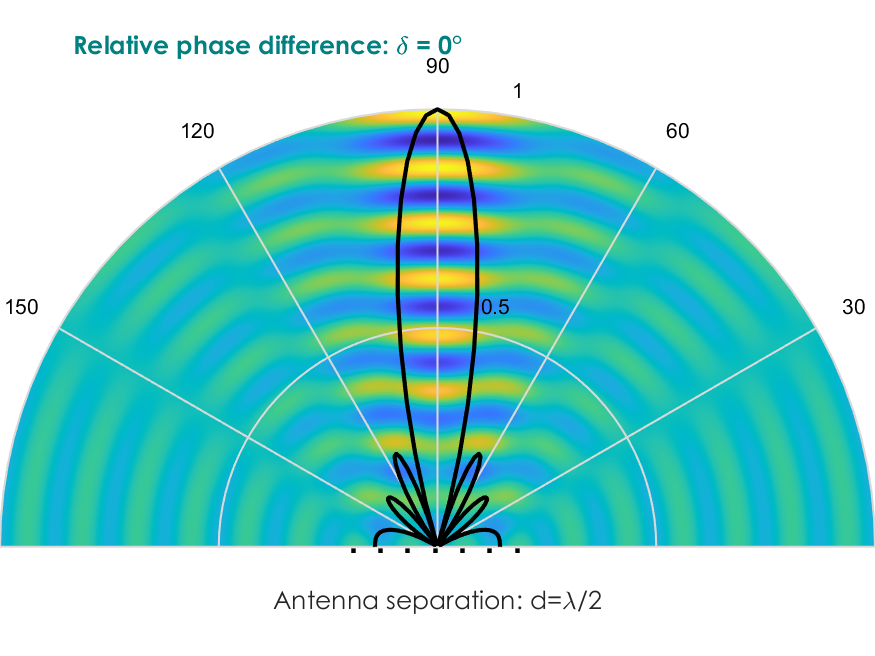
\includegraphics[width=\textwidth]{beam_pattern_delta_0_deg.png}
        \caption{Διάγραμμα ακτινοβολίας για \( \delta = 0^\circ \)}
    \end{minipage}
    \hfill
    \begin{minipage}[b]{0.48\textwidth}
        \centering
        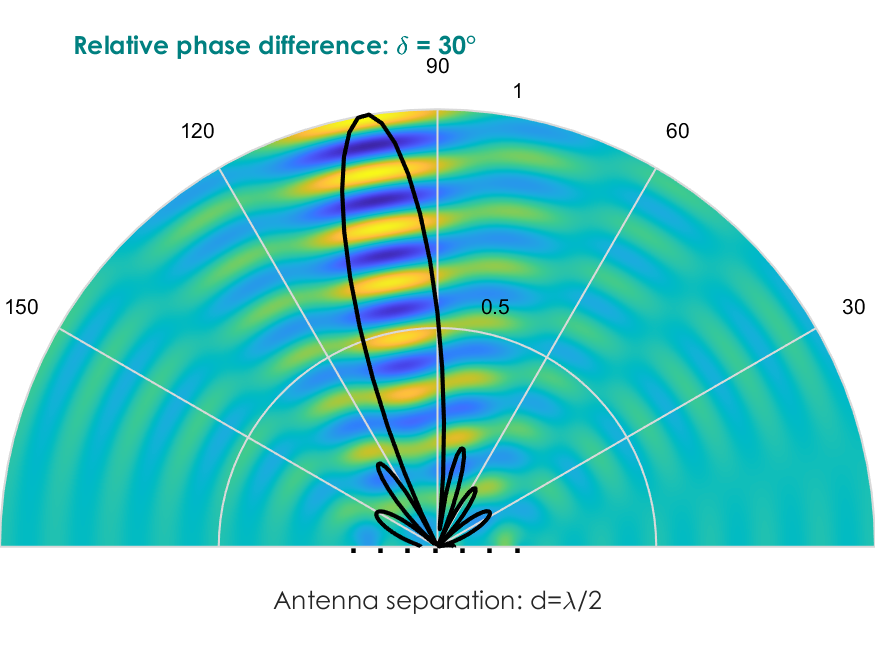
\includegraphics[width=\textwidth]{beam_pattern_delta_30_deg.png}
        \caption{Διάγραμμα ακτινοβολίας για \( \delta = 30^\circ \)}
    \end{minipage}
\end{figure}

\begin{figure}[H]
    \centering
    \begin{minipage}[b]{0.48\textwidth}
        \centering
        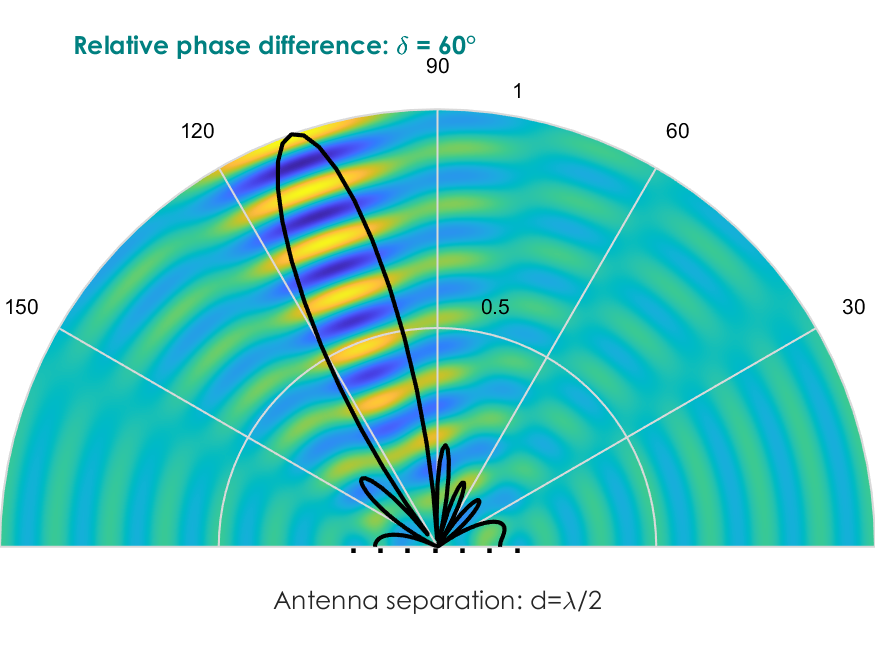
\includegraphics[width=\textwidth]{beam_pattern_delta_60_deg.png}
        \caption{Διάγραμμα ακτινοβολίας για \( \delta = 60^\circ \)}
    \end{minipage}
    \hfill
    \begin{minipage}[b]{0.48\textwidth}
        \centering
        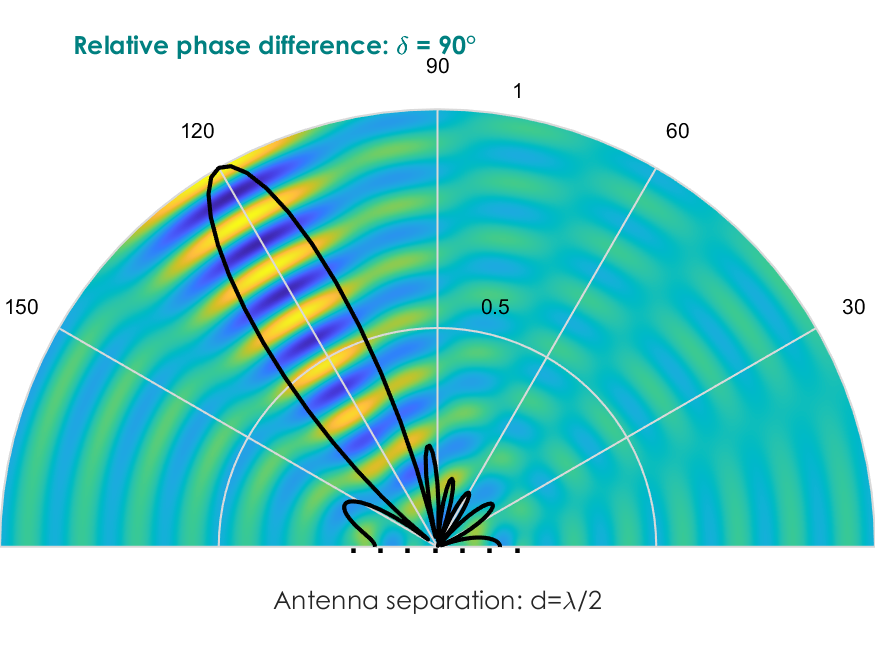
\includegraphics[width=\textwidth]{beam_pattern_delta_90_deg.png}
        \caption{Διάγραμμα ακτινοβολίας για \( \delta = 90^\circ \)}
    \end{minipage}
\end{figure}


\subsubsection{Μελέτη της Επίδρασης του \(\mathbf{d = \frac{\lambda}{4}}\)}

Στο δεύτερο σκέλος της άσκησης, τροποποιήθηκε η απόσταση μεταξύ των στοιχείων σε \( d = \frac{\lambda}{4} \). Οι υπόλοιπες συνθήκες παρέμειναν ίδιες.

\vspace{0.3cm}

\hspace{-0.6cm}Ακολουθούν οι αντίστοιχες απεικονίσεις για τις τέσσερις γωνίες στροφής:

\begin{figure}[H]
    \centering
    \begin{minipage}[b]{0.48\textwidth}
        \centering
        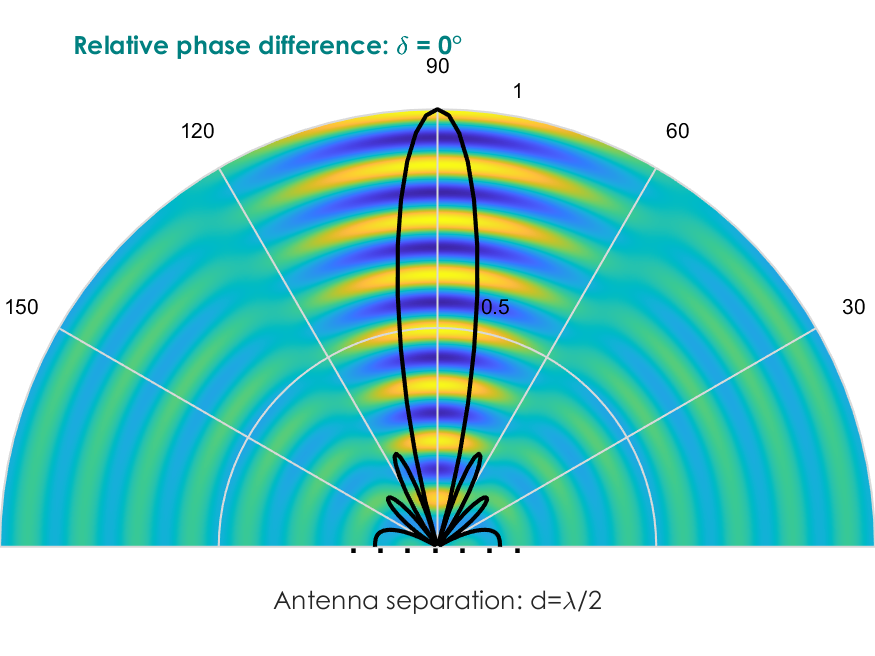
\includegraphics[width=\textwidth]{pattern_delta_Aii_0_deg.png}
        \caption{Διάγραμμα ακτινοβολίας για \( \delta = 0^\circ \), με \( d = \frac{\lambda}{4} \)}
    \end{minipage}
    \hfill
    \begin{minipage}[b]{0.48\textwidth}
        \centering
        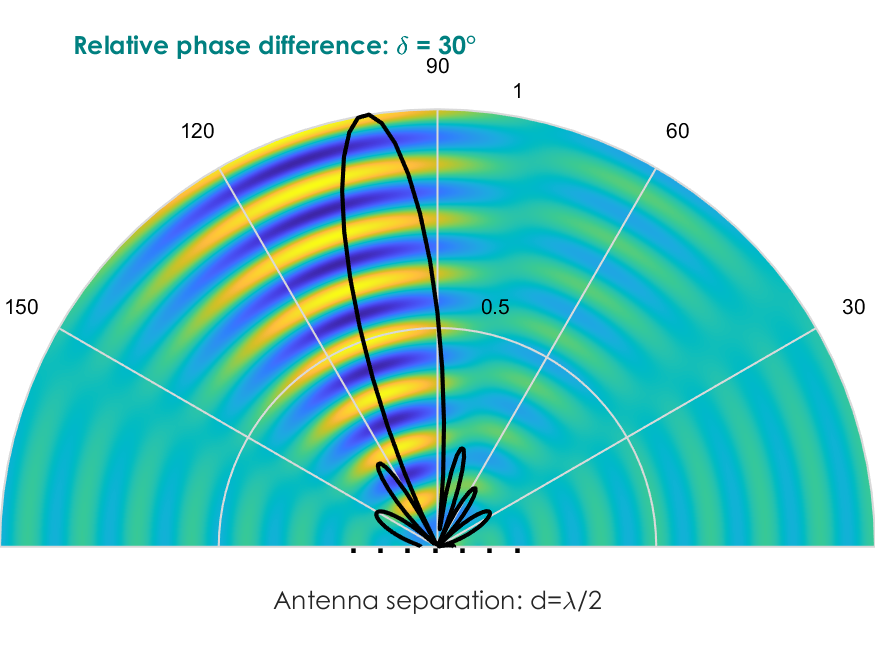
\includegraphics[width=\textwidth]{pattern_delta_Aii_30_deg.png}
        \caption{Διάγραμμα ακτινοβολίας για \( \delta = 30^\circ \), με \( d = \frac{\lambda}{4} \)}
    \end{minipage}
\end{figure}

\begin{figure}[H]
    \centering
    \begin{minipage}[b]{0.48\textwidth}
        \centering
        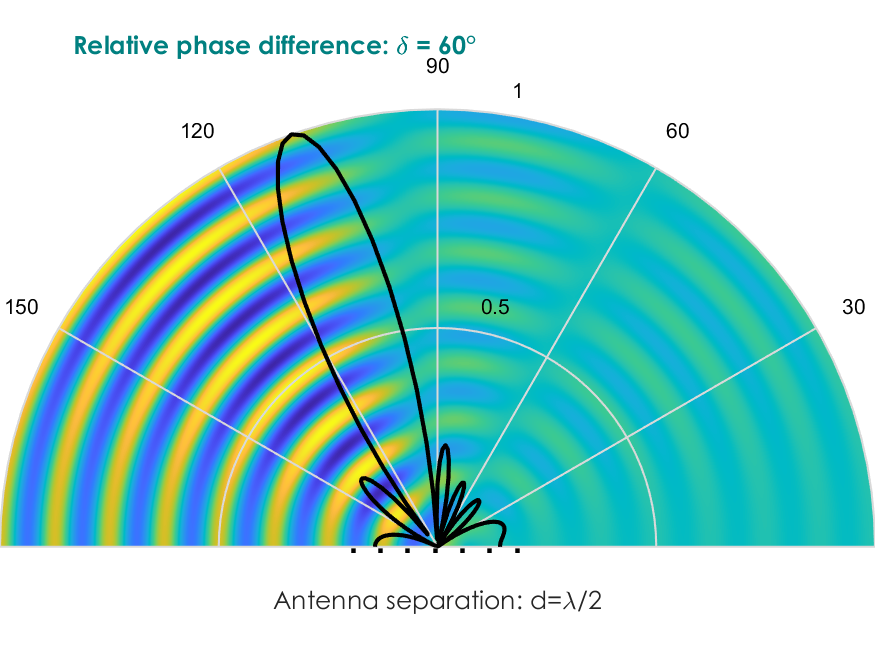
\includegraphics[width=\textwidth]{pattern_delta_Aii_60_deg.png}
        \caption{Διάγραμμα ακτινοβολίας για \( \delta = 60^\circ \), με \( d = \frac{\lambda}{4} \)}
    \end{minipage}
    \hfill
    \begin{minipage}[b]{0.48\textwidth}
        \centering
        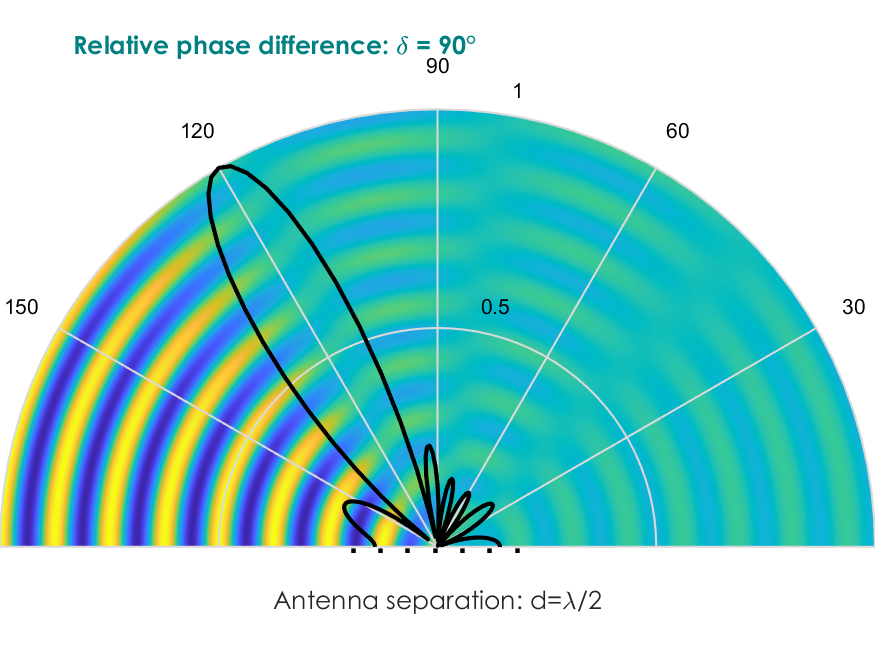
\includegraphics[width=\textwidth]{pattern_delta_Aii_90_deg.png}
        \caption{Διάγραμμα ακτινοβολίας για \( \delta = 90^\circ \), με \( d = \frac{\lambda}{4} \)}
    \end{minipage}
\end{figure}


\subsection{Σύγκριση και Παρατηρήσεις}

Ορισμένες από τις γενικές μου παρατηρήσεις για το ερώτημα αυτό επιδεικνύονται παρακάτω:

\begin{itemize}
    \item Καθώς αυξάνεται η τιμή του \(\delta\), η κατεύθυνση της κύριας δέσμης μετατοπίζεται αντιστοίχως προς τα δεξιά, επιβεβαιώνοντας τη δυνατότητα ελέγχου του λοβού ακτινοβολίας μέσω φασικών μετατοπίσεων.
    \item Η δομή της κεραίας είναι συμμετρική ως προς το κέντρο της, γεγονός που καθιστά την ακτινοβολία επίσης συμμετρική για γωνίες ±\(\theta\).
    \item Σε υψηλότερες γωνίες (όπως \( \theta = 90^\circ \)) μπορεί να παρατηρηθεί αύξηση των πλευρικών λοβών, γεγονός που περιορίζει την καθαρότητα της κατευθυντικότητας.
\end{itemize}

\hspace{-0.6cm}Η σύγκριση των διαγραμμάτων ακτινοβολίας για τις δύο περιπτώσεις απόστασης \( d = \frac{\lambda}{2} \) και \( d = \frac{\lambda}{4} \) αποκαλύπτει τα εξής βασικά σημεία:

\begin{itemize}
    \item \textbf{Για \( d = \frac{\lambda}{2} \):}
    \begin{itemize}
        \item Η κύρια δέσμη είναι στενή και εμφανίζει υψηλή κατευθυντικότητα.
        \item Παρατηρούνται έντονοι πλευρικοί λοβοί, ιδιαίτερα για μεγαλύτερες γωνίες στροφής \( \delta \), γεγονός που μπορεί να οδηγήσει σε ανεπιθύμητη εκπομπή σε δευτερεύουσες κατευθύνσεις.
    \end{itemize}

    \item \textbf{Για \( d = \frac{\lambda}{4} \):}
    \begin{itemize}
        \item Οι πλευρικοί λοβοί μειώνονται αισθητά, ενισχύοντας την καθαρότητα της κύριας δέσμης.
        \item Η κύρια δέσμη γίνεται πλατύτερη, υποδεικνύοντας μικρότερη κατευθυντικότητα.
        \item Δεν εμφανίζονται φαινόμενα ψευδολοβών (\en grating lobes\gr), τα οποία τείνουν να προκύπτουν όταν \( d > \frac{\lambda}{2} \).
    \end{itemize}

    \item \textbf{Επίδραση της φασικής διαφοράς \( \delta \):}
    \begin{itemize}
        \item Η κύρια δέσμη μετατοπίζεται σε γωνία ίση με την αντίστοιχη τιμή του \( \delta \), ανεξαρτήτως της απόστασης \( d \), επιβεβαιώνοντας την ικανότητα κατεύθυνσης της ακτινοβολίας μέσω φασικών μετατοπίσεων.
    \end{itemize}

    \item \textbf{Συμπερασματικά:}
    \begin{itemize}
        \item Η επιλογή της τιμής του \( d \) επηρεάζει τον συμβιβασμό μεταξύ κατευθυντικότητας και καθαρότητας ακτινοβολίας.
        \item Το \( d = \frac{\lambda}{2} \) είναι κατάλληλο για εφαρμογές που απαιτούν υψηλή κατευθυντικότητα.
        \item Το \( d = \frac{\lambda}{4} \) ενδείκνυται όταν προτιμάται η μείωση των πλευρικών λοβών, ακόμα και εις βάρος της οξύτητας της δέσμης.
    \end{itemize}
\end{itemize}

\vspace{0.2cm}

\hspace{-0.6cm}Οι αντίστοιχοι κώδικες για το Ερώτημα Α βρίσκονται στα αρχεία \en \texttt{Exercise1Ai.m} \gr και \en \texttt{Exercise1Aii.m}\gr, αντίστοιχα.

\vspace{0.5cm}

\section{Ανάλυση Σκέλους B: Επίδραση Αριθμού Στοιχείων στη Δέσμη}

Το δεύτερο σκέλος της άσκησης μελετά την επίδραση του πλήθους των στοιχείων σε μια γραμμική ομοιόμορφη στοιχειοκεραία στο πρότυπο ακτινοβολίας. Συγκεκριμένα, εξετάζονται δύο περιπτώσεις με \( N = 5 \) και \( N = 9 \) στοιχεία, διατηρώντας την ίδια απόσταση \( d = \frac{\lambda}{2} \) μεταξύ τους και λειτουργία στη συχνότητα \( f = 1 \text{\en GHz\gr} \).

\subsection{Περιγραφή Προσομοίωσης}

Η προσομοίωση πραγματοποιήθηκε και εδώ στο \en MATLAB\gr, με τις εξής βασικές ενέργειες:

\begin{itemize}
    \item Ορίζονται παραμετρικά οι δύο διαμορφώσεις στοιχειοκεραίας με 5 και 9 στοιχεία, με συμμετρική διάταξη ως προς το κέντρο.
    \item Για κάθε περίπτωση, εφαρμόζεται στροφή δέσμης για δύο διαφορετικές φασικές μετατοπίσεις \( \delta \) της επιλογής μας (ενδεικτικά: \( 60^\circ \) και \( 120^\circ \)).
    \item Υπολογίζεται το πεδίο από κάθε στοιχείο της διάταξης στο δισδιάστατο επίπεδο παρατήρησης για χρονική στιγμή \( t = 0 \).
    \item Τα πεδία υπερτίθενται, ενώ παράλληλα υπολογίζεται και ο παράγοντας της στοιχειοκεραίας.
    \item Παράγονται διαγράμματα τόσο της κατανομής του πεδίου όσο και του array factor σε πολική μορφή.
\end{itemize}

\subsection{Ανάλυση Κώδικα Υλοποίησης}

Το παρακάτω τμήμα παρουσιάζει τον ψευδοκώδικα για την προσομοίωση του Σκέλους B:

\begin{tcolorbox}[colback=gray!5!white, colframe=black!75!black, title=Ψευδοκώδικας \en \texttt{BeamRotation\_MultiSize} \gr]

\en
\begin{verbatim}
1. Define freq, lambda, k, T, spatial and temporal steps.
2. Create (x, y) observation grid in polar form.
3. Define array_sizes = [5, 9]
4. Set steering phase angles:
       deltaAll = [0, pi/3, pi/2, 2*pi/3]
5. For each number of elements in array_sizes:
    a. Define symmetrical element positions along x-axis.
    b. For each delta in deltaAll:
        i. For each grid point (x,y):
            - Compute distance Rn from each element
            - Compute field: En(x,y) = cos(omega*t - k·Rn + n*delta)
        ii. Superpose all fields: E = sum(En)
        iii. Compute array factor Fa(theta)
        iv. Normalize and plot Fa(theta), E(x,y)
\end{verbatim}
\gr
\end{tcolorbox}

\hspace{-0.6cm}Οι μαθηματικές εκφράσεις που εφαρμόζονται είναι παρόμοιες με το Σκέλος Α:

\begin{itemize}
    \item Η χωρική κατανομή πεδίου προκύπτει από τη συνάρτηση:
    \[
    E(x, y) = \sum_{n = -\frac{N-1}{2}}^{\frac{N-1}{2}} \cos(\omega t - k R_n + n \cdot \delta)
    \]
    \item Ο παράγοντας στοιχειοκεραίας ορίζεται ως:
    \[
    Fa(\theta) = \left| \sum_{n=0}^{N-1} A_n \cdot e^{-j n \delta + j k (n d - d_c) \cos(\theta)} \right|
    \]
    όπου \( d_c = \frac{(N-1)}{2}d \) και \( A_n = 1 \) (ομοιόμορφη ενίσχυση).
    \item Οι γωνίες φασικής μετατόπισης επιλέχθηκαν ως:
    \[
    \delta \in \left\{ 0, \frac{\pi}{3}, \frac{\pi}{2}, \frac{2\pi}{3} \right\}
    \]
\end{itemize}

\subsection{Απεικονίσεις και οπτικοποίηση αποτελεσμάτων κώδικα}

Οι παρακάτω εικόνες παρουσιάζουν τις γραφικές παραστάσεις του πεδίου και του array factor για τις περιπτώσεις \( N = 5 \) και \( N = 9 \) στοιχείων, με φασική μετατόπιση \( \delta \) ίση με \( 60^\circ \) και \( 120^\circ \).

\begin{figure}[H]
\centering
\begin{minipage}{0.48\textwidth}
    \centering
    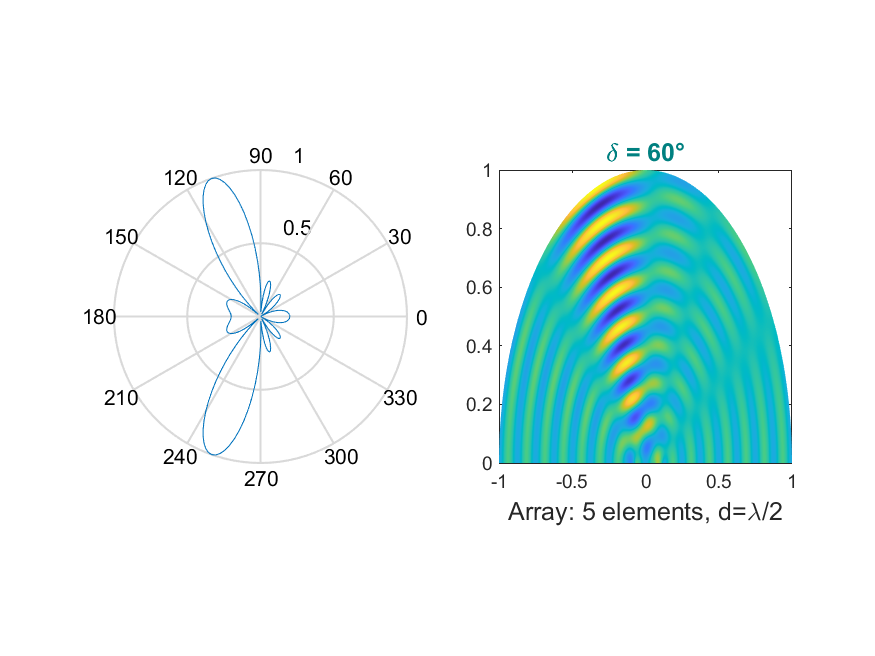
\includegraphics[width=\textwidth]{beta_pattern_5elems_delta_60_deg.png}
    \caption{Απεικόνηση για \(N=5\), \(\delta=60^\circ\)}
\end{minipage}
\hfill
\begin{minipage}{0.48\textwidth}
    \centering
    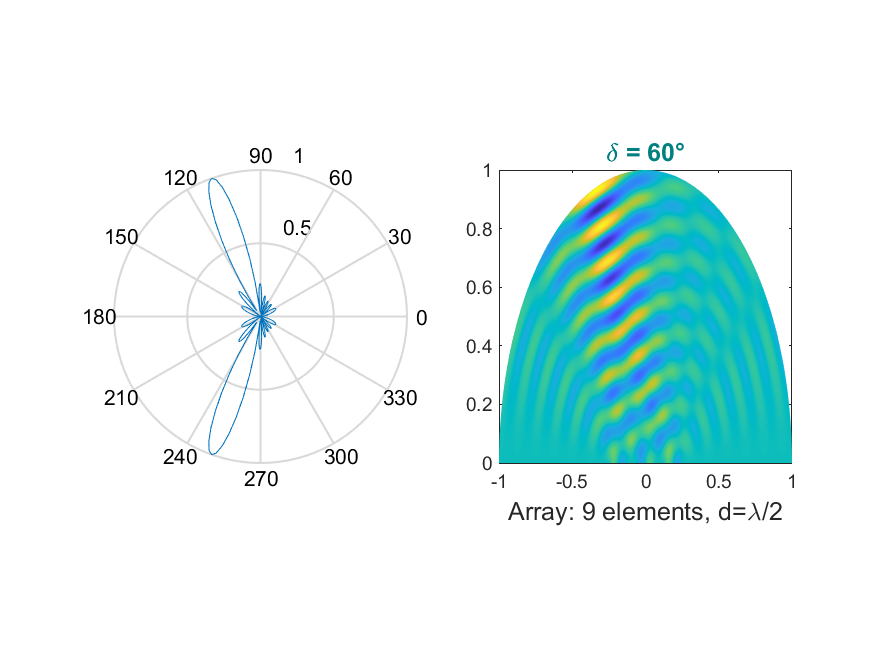
\includegraphics[width=\textwidth]{beta_pattern_9elems_delta_60_deg.png}
    \caption{Απεικόνηση για \(N=9\), \(\delta=60^\circ\)}
\end{minipage}
\vspace{0.3cm}
\begin{minipage}{0.48\textwidth}
    \centering
    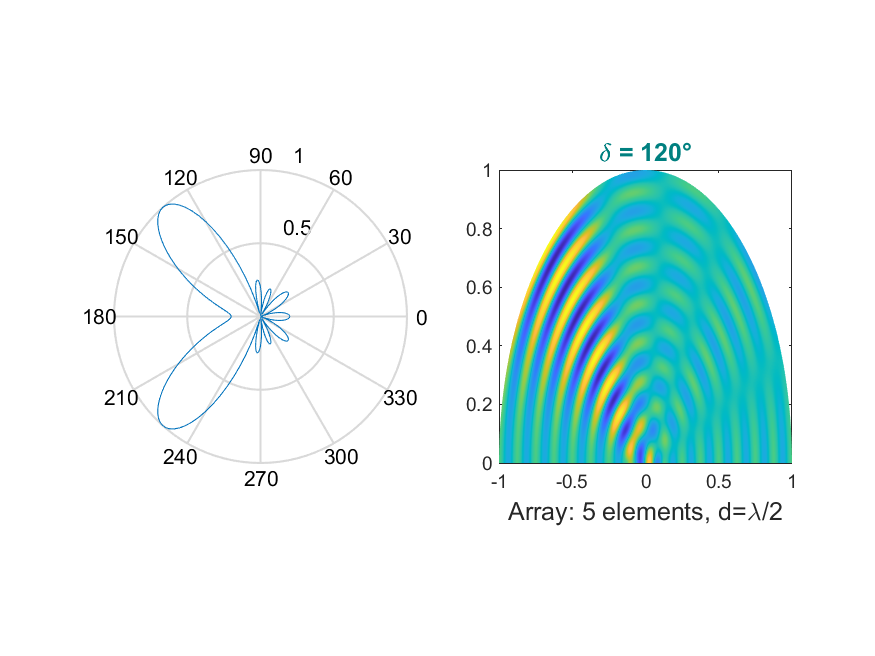
\includegraphics[width=\textwidth]{beta_pattern_5elems_delta_120_deg.png}
    \caption{Απεικόνηση για \(N=5\), \(\delta=120^\circ\)}
\end{minipage}
\hfill
\begin{minipage}{0.48\textwidth}
    \centering
    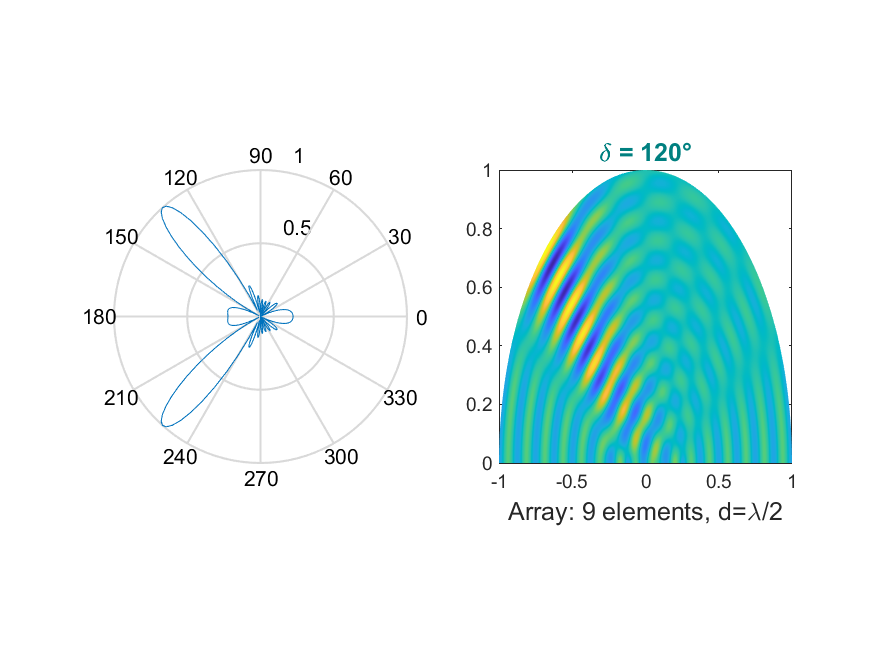
\includegraphics[width=\textwidth]{beta_pattern_9elems_delta_120_deg.png}
    \caption{Απεικόνηση για \(N=9\), \(\delta=120^\circ\)}
\end{minipage}
\end{figure}

\subsection{Παρατηρήσεις και συμπεράσματα}

Από τη σύγκριση των προσομοιώσεων για \( N = 5 \) και \( N = 9 \) στοιχεία, καθώς και για δύο γωνίες στροφής δέσμης (\( \delta = 60^\circ \) και \( \delta = 120^\circ \)), προκύπτουν τα εξής συμπεράσματα:

\begin{itemize}
    \item \textbf{Επίδραση αριθμού στοιχείων (5 έναντι 9):}
    \begin{itemize}
        \item Η αύξηση του αριθμού των στοιχείων από \( N = 5 \) σε \( N = 9 \) οδηγεί σε σημαντική στένωση της κύριας δέσμης, κάτι που υποδηλώνει αυξημένη κατευθυντικότητα.
        \item Οι πλευρικοί λοβοί εμφανίζονται περισσότερο κατασταλμένοι στην περίπτωση των 9 στοιχείων, καθιστώντας τη δέσμη πιο καθαρή και εστιασμένη.
        \item Η δέσμη των 5 στοιχείων είναι ευρύτερη, γεγονός που μειώνει την ακρίβεια προσανατολισμού και επιτρέπει μεγαλύτερη διαρροή ενέργειας σε μη επιθυμητές διευθύνσεις.
    \end{itemize}

    \item \textbf{Επίδραση στροφής φάσης \( \delta \):}
    \begin{itemize}
        \item Η μεταβολή της φασικής διαφοράς \( \delta \) επιτρέπει την προσαρμογή της διεύθυνσης ακτινοβολίας της κύριας δέσμης, χωρίς να μετακινείται φυσικά η κεραία.
        \item Όσο αυξάνεται το \( \delta \), τόσο περισσότερο μετατοπίζεται η δέσμη προς μεγαλύτερες γωνίες (σε συμφωνία με τη θεωρία του ηλεκτρονικού σαρώματος).
        \item Ωστόσο, για μεγαλύτερες τιμές \( \delta \), εμφανίζονται εντονότεροι πλευρικοί λοβοί, ειδικά στην περίπτωση των 5 στοιχείων.
    \end{itemize}

    \item \textbf{Συγκεντρωτικά:}
    \begin{itemize}
        \item Ο αριθμός των στοιχείων επηρεάζει άμεσα την κατευθυντικότητα, την καταστολή πλευρικών λοβών και την εστίαση της ενέργειας.
        \item Η κατάλληλη επιλογή του πλήθους στοιχείων και της γωνίας στροφής \( \delta \) επιτρέπει τον ακριβή έλεγχο της διαμόρφωσης της δέσμης.
    \end{itemize}
\end{itemize}

\vspace{0.2cm}

\hspace{-0.6cm}Ο αντίστοιχος κώδικας με σχόλια και παρατηρήσεις βρίσκεται στο αρχείο \en \texttt{Exercise1B.m}\gr.

\vspace{0.5cm}

\section{Ανάλυση Σκέλους Γ: Διωνυμική Κατανομή σε Στοιχειοκεραία}

Το τρίτο σκέλος της άσκησης εξετάζει την εφαρμογή διωνυμικής κατανομής βαρών \en (binomial tapering) \gr σε μια ομοιόμορφη γραμμική στοιχειοκεραία επτά στοιχείων, με στόχο τον έλεγχο του πλάτους της κύριας δέσμης και την καταστολή των πλευρικών λοβών. Η κεραία λειτουργεί στη συχνότητα \( f = 1\, \text{\en GHz\gr} \), με σταθερή απόσταση μεταξύ των στοιχείων \( d = \frac{\lambda}{2} \).

\subsection{Περιγραφή Προσομοίωσης}

Η υλοποίηση πραγματοποιείται σε περιβάλλον \en MATLAB\gr, με τα ακόλουθα βασικά βήματα:

\begin{itemize}
    \item Καθορισμός χωρικών και χρονικών βημάτων, καθώς και δημιουργία πολικής περιοχής παρατήρησης \((R, \theta)\).
    \item Υπολογισμός των διωνυμικών συντελεστών βαρών \( A_n \) για \( N = 7 \) στοιχεία, βάσει του τύπου:
    \[
    A_n = \frac{ \binom{N-1}{n} }{ \sum_{k=0}^{N-1} \binom{N-1}{k} }
    \]
    \item Υπολογισμός του συνολικού ηλεκτρικού πεδίου σε κάθε σημείο του χώρου από όλα τα στοιχεία, λαμβάνοντας υπόψη τις σχετικές φάσεις.
    \item Υπολογισμός και σχεδίαση του \en array factor \gr \( Fa(\theta) \), για τέσσερις διαφορετικές γωνίες στροφής \( \delta \in \{0^\circ, 60^\circ, 90^\circ, 120^\circ\} \).
\end{itemize}

\subsection{Ανάλυση Κώδικα Υλοποίησης}

Ακολουθεί σύνοψη του ψευδοκώδικα όπως εφαρμόστηκε στο σκέλος Γ:

\begin{tcolorbox}[colback=gray!5!white, colframe=black!75!black, title=Ψευδοκώδικας \en \texttt{Binomial\_Array\_Sim} \gr]
\en
\begin{verbatim}
1. Define parameters: freq, lambda, k, T, sampling in space/time
2. Construct spatial grid (x, y) in polar coordinates
3. Define array size (e.g. 7 elements), spacing d = lambda/2
4. Compute binomial weights A = nchoosek(N-1, n)/sum(...)
5. For each delta in [0, pi/3, pi/2, 2*pi/3]:
    a. For each element:
        i. Define position x_n
        ii. Compute phase shift phi_n = delta*(n - mid)
        iii. For all grid points: add weighted field
             E += A(n) * cos(omega*t - k*R + phi_n)
    b. Compute array factor:
        Fa(theta) = |sum A(n) * exp(-j*n*delta + j*k*(x_n)*cos(theta))|
    c. Normalize and plot Fa(theta), E(x,y)
\end{verbatim}
\gr
\end{tcolorbox}

\subsection{Μαθηματικές Εκφράσεις}
Και σε αυτό το ερώτημα οι εκφράσεις του συνολικού πεδίου και του παράγοντα στοιχειοκεραίας είναι οι παρακάτω:

\begin{itemize}
    \item Συνολικό πεδίο:
    \[
    E(x, y) = \sum_{n=0}^{N-1} A_n \cdot \cos\left( \omega t - k R_n + \phi_n \right)
    \]
    \item Παράγοντας στοιχειοκεραίας (με βάρη \( A_n \)):
    \[
    Fa(\theta) = \left| \sum_{n=0}^{N-1} A_n \cdot e^{-j n \delta + j k (n - d_c) d \cos(\theta)} \right|
    \]
    όπου \( d_c = \frac{(N-1)}{2} \), δηλαδή το μέσο στοιχείο.
\end{itemize}

\subsection{Απεικονίσεις και Οπτικοποίηση}

Για την οπτική αξιολόγηση των αποτελεσμάτων, υλοποιήθηκε γραφική απεικόνιση τόσο του \en array factor \gr (πολικό διάγραμμα), όσο και της κατανομής του ηλεκτρικού πεδίου στον χώρο για κάθε μία από τις τέσσερις γωνίες στροφής της δέσμης: \( \delta = 0^\circ, 60^\circ, 90^\circ, 120^\circ \).

\vspace{0.3cm}

\hspace{-0.6cm}Η προσομοίωση βασίστηκε στην διαδικασία που παρουσιάστηκε αναλυτικά και παραπάνω. Παρακάτω παρουσιάζονται οι απεικονήσεις ενδεικτικών παραδειγμάτων. Πιο συγκεκριμένα επιδεικνύονται οι απεικονίσεις \en array factor \gr και κατανομής πεδίου για 7 στοιχεία με διωνυμική κατανομή και διάφορες γωνίες στροφής.

\begin{figure}[H]
    \centering
    \begin{minipage}[t]{0.48\textwidth}
        \centering
        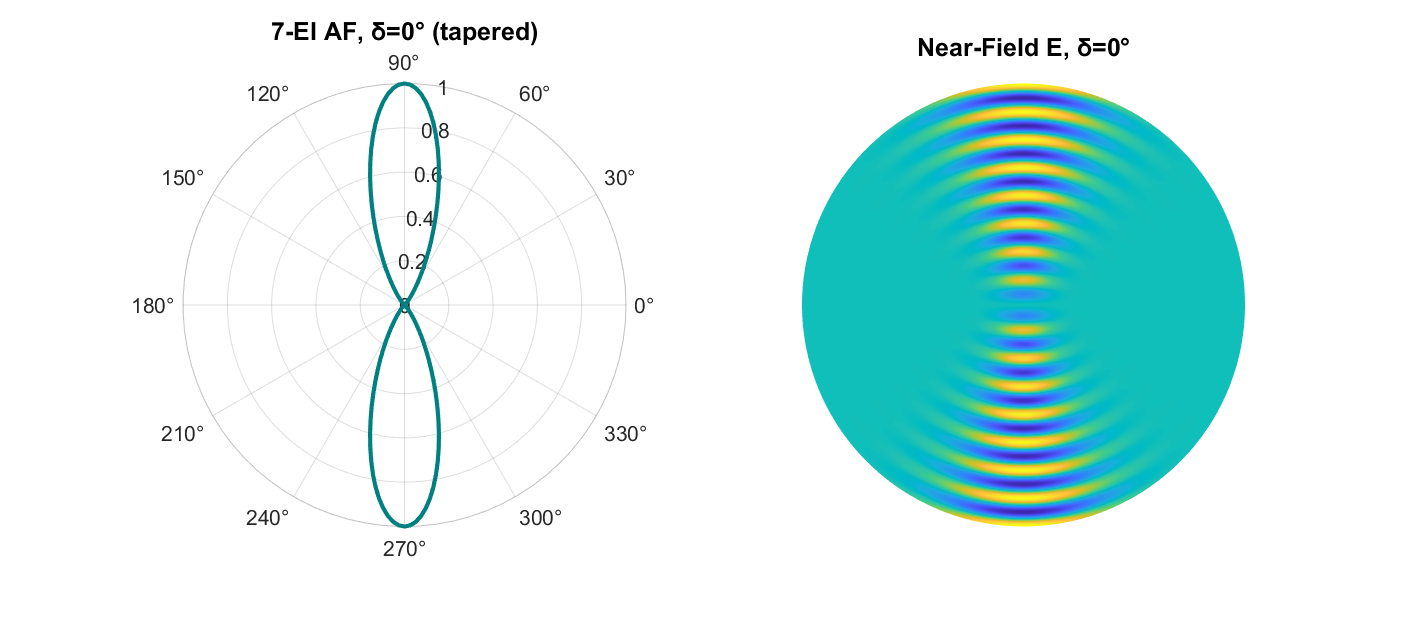
\includegraphics[width=\textwidth]{binomial_pattern_7elems_delta_0_deg.png}
        \caption{Απεικόνιση για \( \delta = 0^\circ \)}
    \end{minipage}
    \hfill
    \begin{minipage}[t]{0.48\textwidth}
        \centering
        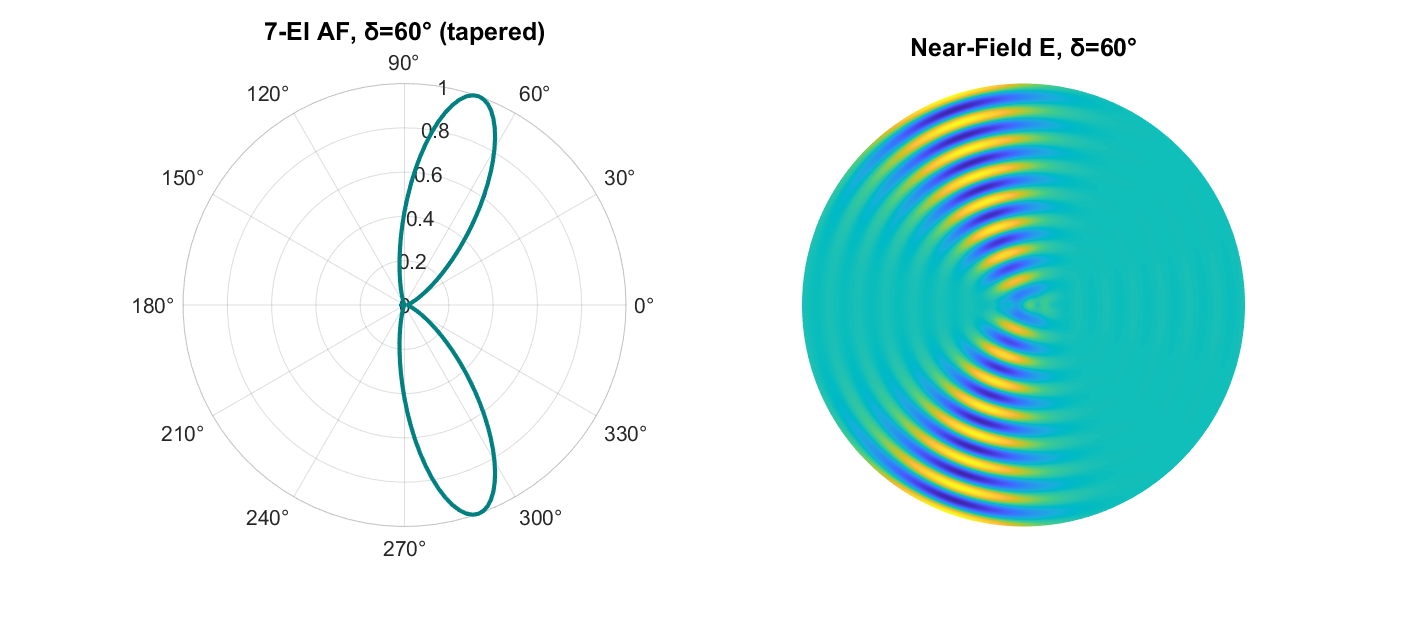
\includegraphics[width=\textwidth]{binomial_pattern_7elems_delta_60_deg.png}
        \caption{Απεικόνιση για \( \delta = 60^\circ \)}
    \end{minipage}

    \vspace{0.4cm}

    \begin{minipage}[t]{0.48\textwidth}
        \centering
        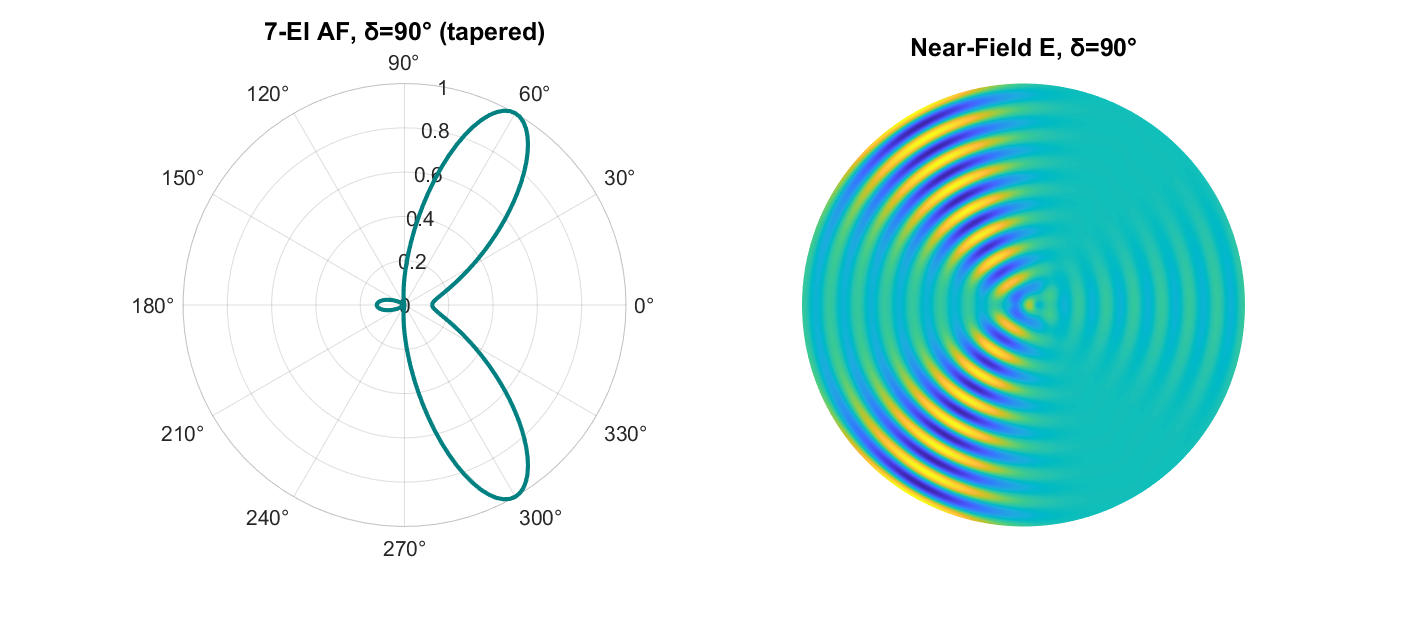
\includegraphics[width=\textwidth]{binomial_pattern_7elems_delta_90_deg.png}
        \caption{Απεικόνιση για \( \delta = 90^\circ \)}
    \end{minipage}
    \hfill
    \begin{minipage}[t]{0.48\textwidth}
        \centering
        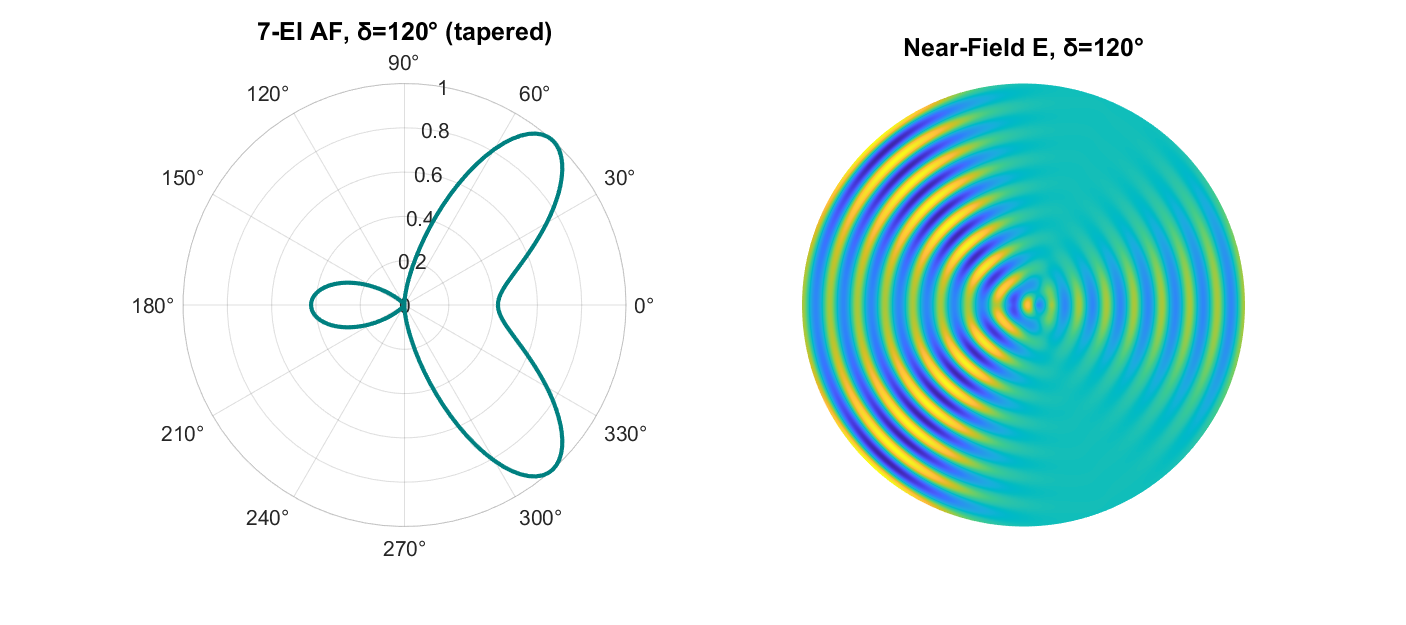
\includegraphics[width=\textwidth]{binomial_pattern_7elems_delta_120_deg.png}
        \caption{Απεικόνιση για \( \delta = 120^\circ \)}
    \end{minipage}
\end{figure}

\subsection{Παρατηρήσεις και Συμπεράσματα}

Το τρίτο σκέλος της εργασίας εξετάζει την εφαρμογή διωνυμικής κατανομής πλάτους σε γραμμική στοιχειοκεραία επτά στοιχείων, με σκοπό τον έλεγχο του εύρους και της μορφής της κύριας δέσμης καθώς και την καταστολή των πλευρικών λοβών.

\vspace{0.3cm}

\hspace{-0.6cm}Η ανάλυση πραγματοποιήθηκε για τέσσερις διαφορετικές γωνίες στροφής \(\delta = 0^\circ, 60^\circ, 90^\circ, 120^\circ\). Τα αποτελέσματα, όπως απεικονίζονται στα Σχήματα 2.13 με 2.16, καταδεικνύουν τα εξής:

\begin{itemize}
    \item Η εφαρμογή διωνυμικών βαρών μειώνει σημαντικά τους πλευρικούς λοβούς (side lobes), προσδίδοντας καλύτερη καταστολή τους σε σύγκριση με ομοιόμορφα βάρη \en (A\textsubscript{n} = 1)\gr.
    \item Η κύρια δέσμη είναι πιο ευρεία (δηλαδή λιγότερο κατευθυντική) λόγω της χαμηλότερης ενίσχυσης στα εξωτερικά στοιχεία της κεραίας.
    \item Για \(\delta = 0^\circ\), η ακτινοβολία είναι συγκεντρωμένη κατά μήκος του κατακόρυφου άξονα με ομαλή απόσβεση.
    \item Καθώς αυξάνεται η τιμή της γωνίας \(\delta\), παρατηρείται στροφή της κύριας δέσμης, η οποία ακολουθεί την επιθυμητή κατεύθυνση με καλή ευστάθεια ως προς τη μορφή του λοβού.
    \item Η ακτινοβολία στο κοντινό πεδίο είναι πιο μαλακή και ομαλή, γεγονός που την καθιστά κατάλληλη για εφαρμογές που απαιτούν χαμηλούς λοβούς πλευρικής ακτινοβολίας, όπως επικοινωνίες σε περιβάλλον με υψηλές απαιτήσεις εμπλοκής.
\end{itemize}

\hspace{-0.6cm}Συμπερασματικά, η χρήση διωνυμικών βαρών σε γραμμικές στοιχειοκεραίες προσφέρει έναν αποδοτικό συμβιβασμό μεταξύ κατευθυντικότητας και καταστολής πλευρικών λοβών. Η προσαρμογή των βαρών επιτρέπει βελτιστοποίηση ανάλογα με τις απαιτήσεις της εφαρμογής, ιδίως όταν η 
καθαρότητα της κύριας δέσμης είναι κρίσιμη.

\vspace{0.2cm}

\hspace{-0.6cm}Ο αντίστοιχος κώδικας με σχόλια και παρατηρήσεις βρίσκεται στο αρχείο \en \texttt{Exercise1C.m}\gr.

\chapter{Δίκτυο διαμόρφωσης δέσμης φασικής στοχειοκεραίας}

\section{Εισαγωγή στο ζητούμενο}

Η δεύτερη άσκηση επικεντρώνεται στην προσομοίωση ενός οπτικού δικτύου διαμόρφωσης δέσμης για φασική στοιχειοκεραία, το οποίο υλοποιείται με χρήση παθητικών οπτικών στοιχείων, όπως τα συμβολόμετρα τύπου \en Mach-Zehnder \gr και οι φασομετατοπιστές \en (phase shifters)\gr. Το σύστημα αυτό ανήκει στην κατηγορία των \en Optical Phased Arrays (OPA) \gr και έχει τη δυνατότητα σχηματισμού και ηλεκτρονικής στροφής της δέσμης εκπομπής χωρίς την ανάγκη μηχανικής μετακίνησης.

\vspace{0.3cm}

\hspace{-0.6cm}Στην εκφώνηση, δίνεται ένα δίκτυο τύπου 1:8, το οποίο αποτελείται από μία οπτική είσοδο και οκτώ εξόδους που καταλήγουν σε ισάριθμα στοιχεία μιας γραμμικής στοιχειοκεραίας. Η δέσμη καθορίζεται μέσω της εισαγωγής φασικών μετατοπίσεων στα μονοπάτια των σημάτων, οι οποίες ρυθμίζονται από κατάλληλους φασομετατοπιστές σε κάθε διαδρομή. Οι φάσεις αυτές εξαρτώνται από τη γωνία στροφής της επιθυμητής δέσμης ακτινοβολίας και μπορούν να υπολογιστούν θεωρητικά με βάση το γεωμετρικό μοντέλο του παράγοντα της στοιχειοκεραίας.

\vspace{0.3cm}

\hspace{-0.6cm}Η προσομοίωση έχει ως στόχο:

\begin{itemize}
    \item Τον υπολογισμό και την εφαρμογή των κατάλληλων φασικών μετατοπίσεων που απαιτούνται για την επίτευξη μέγιστης ενίσχυσης της δέσμης σε επιλεγμένες γωνίες κατεύθυνσης (π.χ. \(30^\circ\), \(60^\circ\), \(90^\circ\)).
    \item Την οπτικοποίηση των παραγόντων της στοιχειοκεραίας για τις παραπάνω γωνίες, βάσει των θεωρητικών τιμών των φάσεων.
    \item Τη μελέτη της δυνατότητας εφαρμογής διωνυμικής κατανομής πλάτους στις τροφοδοσίες, ώστε να μειωθούν τα πλευρικά λοβοειδή και να βελτιωθεί η κατευθυντικότητα του συστήματος.
\end{itemize}

\hspace{-0.6cm}Η προσέγγιση ακολουθεί παρόμοια λογική με εκείνη της άσκησης 1, ωστόσο διαφοροποιείται στον τρόπο δημιουργίας της διαμόρφωσης. Ενώ στην πρώτη άσκηση οι φάσεις εφαρμόζονται άμεσα μέσω ημιτονοειδών συναρτήσεων πεδίου, εδώ υλοποιούνται βάσει φυσικών φασομετατοπιστών που περιγράφουν οπτικά μονοπάτια. Επιπλέον, χρησιμοποιείται θεωρία γραμμικών στοιχειοκεραιών και παράγοντες στοιχειοκεραίας για την ποσοτική αποτίμηση των αποτελεσμάτων.

\hspace{-0.6cm}Η υλοποίηση των παραπάνω πραγματοποιείται στο περιβάλλον \en \texttt{MATLAB}\gr, όπου γίνεται χρήση πίνακα φάσεων για κάθε επιθυμητή γωνία και υπολογίζεται ο αντίστοιχος παράγοντας στοιχειοκεραίας, με στόχο τη γραφική απεικόνιση και αξιολόγηση της κατευθυντικότητας του συστήματος, την αποτύπωση σε πολικά διαγράμματα το μέτρο του παράγοντα της στοιχειοκεραίας. Επίσης, γίνεται ποιοτική περιγραφή της διαδικασίας που θα ακολουθούσαμε ώστε να εφαρμόστει διωνυμική κατανομή στα πλάτη των σημάτων τροφοδοσίας της στοιχειοκεραίας.

\vspace{0.5cm}

\section{Υλοποίηση Ερωτήματος Α: Στροφή Οπτικής Δέσμης με Φασική Στοιχειοκεραία}

Το πρώτο ερώτημα της Άσκησης 2 επικεντρώνεται στην προσομοίωση του παράγοντα στοιχειοκεραίας \en (array factor) \gr για ένα σύστημα διαμόρφωσης οπτικής δέσμης τύπου 1:8. Συγκεκριμένα, καλούμαστε να εξετάσουμε την επίδραση της φασικής μετατόπισης στα στοιχεία της κεραίας για τρεις διαφορετικές γωνίες στροφής: \(30^\circ\), \(60^\circ\) και \(90^\circ\).

\subsection{Βήματα Προσομοίωσης και Υλοποίησης}
Η υλοποίησή μου σε \en \texttt{MATLAB} \gr για το ερώτημα αυτό απαρτίζεται από μία αλληλουχία από βήματα που παρατίθενται παρακάτω.

\begin{itemize}
  \item Ορίζονται τα βασικά φυσικά μεγέθη: το μήκος κύματος \(\lambda = 1550\,\text{\en nm\gr}\), ο κυμαριθμός \(k = \frac{2\pi}{\lambda}\), και ο αριθμός των στοιχείων \(N = 8\).
  \item Ορίζεται η απόσταση μεταξύ των στοιχείων ως \(d = \frac{\lambda}{2}\).
  \item Για κάθε επιθυμητή γωνία στροφής \(\theta_0\), υπολογίζονται οι απαραίτητες φασικές μετατοπίσεις για κάθε στοιχείο, με βάση τη σχέση:
  \[
  \phi_n = -n k d \sin(\theta_0)
  \]
  \item Με χρήση της παραπάνω φασικής μετατόπισης, υπολογίζεται το \en array factor (AF) \gr ως:
  \[
  AF(\theta) = \left| \sum_{n=0}^{N-1} e^{j k d n (\sin(\theta) - \sin(\theta_0))} \right|
  \]
  \item Το αποτέλεσμα απεικονίζεται πολικά (σε μορφή \en polarplot\gr), επιτρέποντας την άμεση παρατήρηση της στροφής της κύριας δέσμη και επιδεικνύονται σε επόμενη υποενότητα.
\end{itemize}

\subsubsection{Παρουσίαση ψευδοκώδικα}

Η παρακάτω ακολουθία παρουσιάζει τον ψευδοκώδικα της διαδικασίας υπολογισμού και απεικόνισης του παράγοντα κεραίας `\en (array factor) \gr για ένα οπτικό σύστημα διαμόρφωσης δέσμης με 8 στοιχεία:

\begin{tcolorbox}[colback=gray!5!white, colframe=black!75!black, title=Ψευδοκώδικας \en \texttt{OpticalBeamSteering}\gr]
\en
\begin{verbatim}
1. Initialize constants:
   - Speed of light: c = 3e8
   - Wavelength: lambda = 1550e-9
   - Wave number: k = 2 * pi / lambda
   - Number of elements: N = 8
   - Element spacing: d = lambda / 2

2. Define beam steering angles:
   - steer_angles = [30°, 60°, 90°]

3. Discretize observation angles:
   - theta = 0 to 2*pi with 720 samples (0.5° resolution)

4. For each steering angle theta₀:
   a. Compute phase shifts for each element:
      - For n from 0 to N-1:
           Phi_n = -n * k * d * sin(theta₀)

   b. Compute array factor:
      - AF(theta) = sum over n of exp(j*k*d*n*(sin(theta)-sin(theta₀)))

   c. Normalize the AF:
      - AF_mag = abs(AF) / N

   d. Plot polar diagram of the normalized AF

   e. Save figure to file

5. Repeat for all steering angles
\end{verbatim}
\end{tcolorbox}

\vspace{0.2cm}

\subsection{Αποτελέσματα Kώδικα και Aπεικονήσεις}

Το παρακάτω αποτέλεσμα αφορά τις φασικές μετατοπίσεις που υπολογίστηκαν για κάθε στοιχείο της οπτικής στοιχειοκεραίας, για τις γωνίες στροφής \( \theta_0 = 30^\circ, 60^\circ, 90^\circ \):

\begin{table}[H]
\centering
\caption{Φασικές μετατοπίσεις ανά στοιχείο για διαφορετικές γωνίες στροφής}
\en
\begin{tabular}{|c|c|c|c|}
\hline
\textbf{n} & \(\phi_n \) [rad] (30°) & \(\phi_n \) [rad] (60°) & \(\phi_n \) [rad] (90°) \\
\hline
0 & 0.0000 & 0.0000 & 0.0000 \\
1 & -1.5708 & -2.7207 & -3.1416 \\
2 & -3.1416 & -5.4414 & -6.2832 \\
3 & -4.7124 & -8.1621 & -9.4248 \\
4 & -6.2832 & -10.8828 & -12.5664 \\
5 & -7.8540 & -13.6035 & -15.7080 \\
6 & -9.4248 & -16.3242 & -18.8496 \\
7 & -10.9956 & -19.0449 & -21.9911 \\
\hline
\end{tabular}
\gr
\end{table}

\hspace{-0.6cm}Οι αντίστοιχες πολικές απεικονίσεις του κανονικοποιημένου παράγοντα στοιχειοκεραίας \(AF(\theta)\), για τις παραπάνω γωνίες στροφής, παρουσιάζονται παρακάτω. Παρατηρείται καθαρή μετατόπιση της κύριας δέσμης προς τη γωνία διεύθυνσης \(\theta_0\), όπως έχει οριστεί από τη φασική μετατόπιση. Οι πολικές απεικονίσεις του παράγοντα στοιχειοκεραίας για διαφορετικές γωνίες στροφής παρουσιάζονται παρακάτω.

\begin{figure}[H]
    \centering
    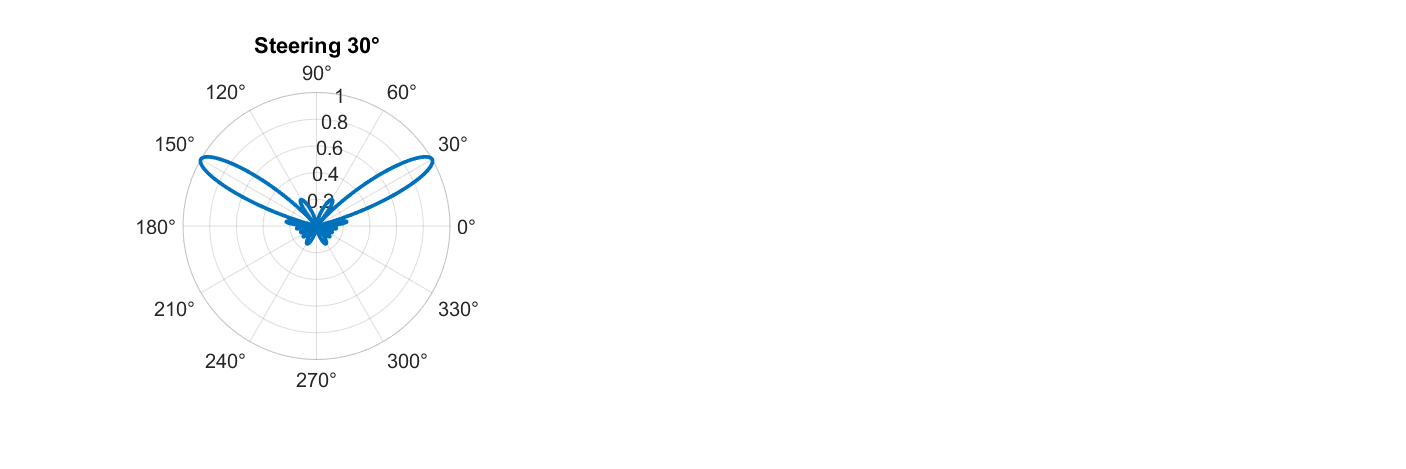
\includegraphics[width=0.95\textwidth]{AF_optical_steering_30_deg.png}
    \caption{Στροφή \( \theta_0 = 30^\circ \)}
\end{figure}

\begin{figure}[H]
    \centering
    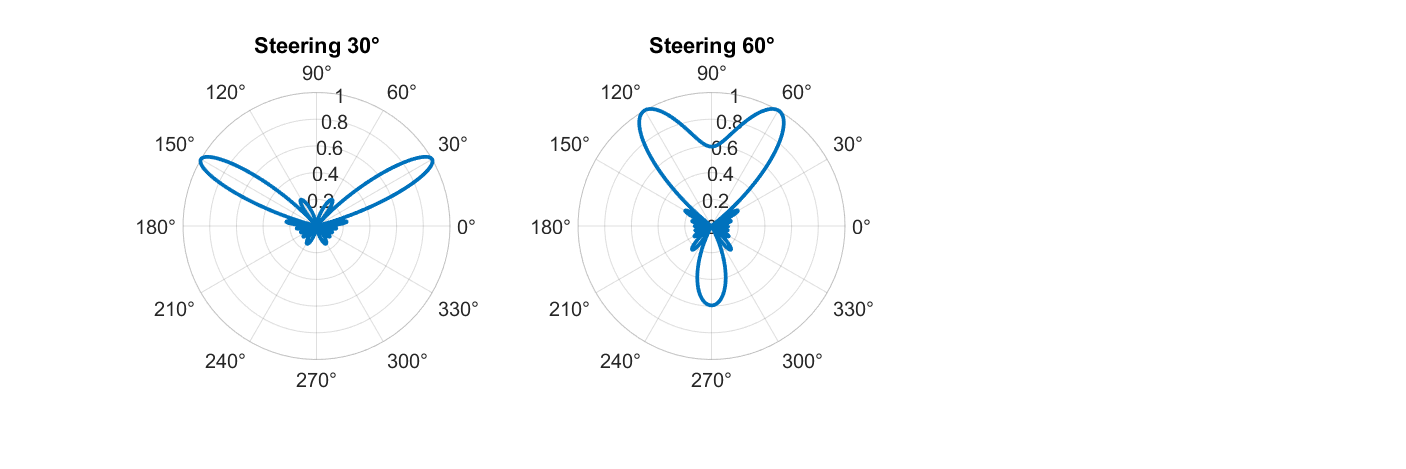
\includegraphics[width=0.95\textwidth]{AF_optical_steering_60_deg.png}
    \caption{Προσθήκη στροφής \( \theta_0 = 60^\circ \)}
\end{figure}

\begin{figure}[H]
    \centering
    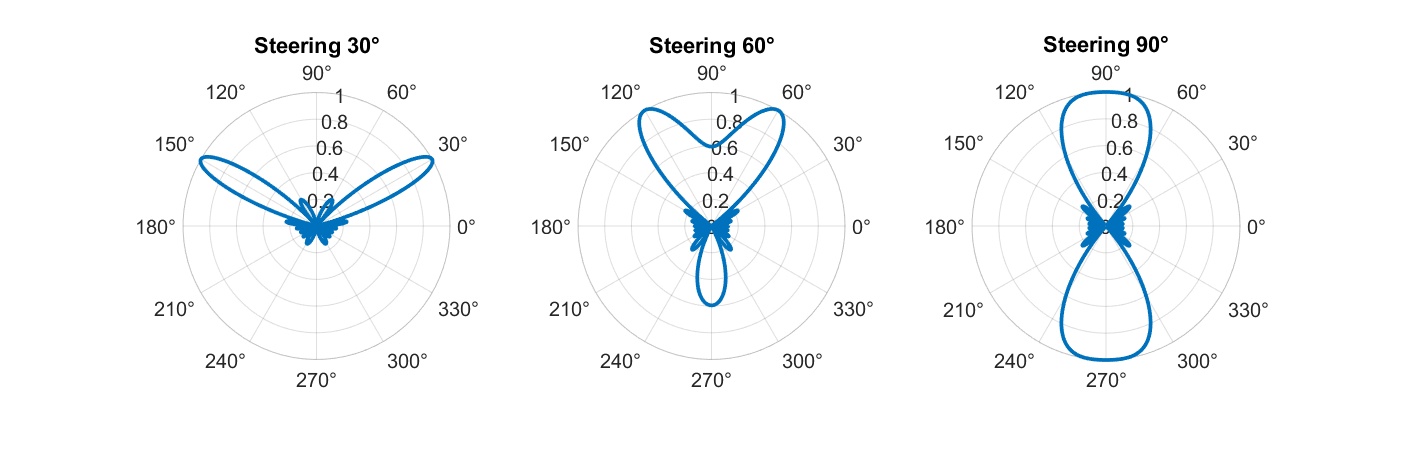
\includegraphics[width=0.95\textwidth]{AF_optical_steering_90_deg.png}
    \caption{Προσθήκη στροφής \( \theta_0 = 90^\circ \)}
\end{figure}

\subsection{Παρατηρήσεις και Συμπεράσματα}
Από τα αποτελέσματα της προσομοίωσης για το ερώτημα Α, παρατηρούμε ότι ο παράγοντας στοιχειοκεραίας \( AF(\theta) \) πράγματι μεγιστοποιείται προς την επιθυμητή γωνία στροφής \( \theta_0 \), όπως προσδιορίζεται από την επιλογή της φασικής μετατόπισης για κάθε στοιχείο. Οι πολικές απεικονίσεις επαληθεύουν την απόκριση του συστήματος και την επιθυμητή κατευθυντικότητα της δέσμης. Για τις διάφορες τιμές των \( \theta_0 \) παρατηρήθηκαν τα παρακάτω: 

\begin{itemize}
    \item Για \( \theta_0 = 30^\circ \), η κύρια δέσμη είναι στραμμένη σαφώς προς την επιθυμητή γωνία, με συμμετρική κατανομή πλευρικών λοβών.
    \item Για \( \theta_0 = 60^\circ \), η κύρια δέσμη μετατοπίζεται προς τα επάνω στον πολικό χάρτη, αποδεικνύοντας την επιτυχία της αλλαγής φάσης.
    \item Για \( \theta_0 = 90^\circ \), η κύρια δέσμη προσανατολίζεται κάθετα προς την κεραία, όπως αναμένεται, εμφανίζοντας διπλή κύρια δέσμη λόγω συμμετρίας.
\end{itemize}

\hspace{-0.6cm}Συνολικά, η υλοποίηση της μεθόδου αποδεικνύει ότι η διαμόρφωση δέσμης μέσω φασικής ολίσθησης αποτελεί μια αξιόπιστη και προβλέψιμη τεχνική για τη δρομολόγηση της ακτινοβολίας στις επιθυμητές διευθύνσεις, συμβάλλοντας στον σχεδιασμό αποδοτικών οπτικών κεραίων.

\vspace{0.5cm}

\section{Ποιοτική Περιγραφή Διωνυμικής Κατανομής Πλάτους}

Για την υλοποίηση μιας διωνυμικής κατανομής στα πλάτη των σημάτων τροφοδοσίας μιας στοιχειοκεραίας, στόχος είναι η σταδιακή αποδυνάμωση των ακραίων στοιχείων και η ενίσχυση των κεντρικών. Αυτή η προσέγγιση μειώνει τους πλευρικούς λοβούς \en (side lobes) \gr του παραγόμενου διαγράμματος ακτινοβολίας, οδηγώντας σε πιο καθαρή κύρια δέσμη.

\subsection{Διαδικασία Εφαρμογής της Διωνυμικής Κατανομής}

\begin{enumerate}
    \item Επιλέγουμε το πλήθος \( N \) των στοιχείων της στοιχειοκεραίας (π.χ. \( N = 8 \)).
    
    \item Υπολογίζουμε τους συντελεστές της διωνυμικής κατανομής μέσω του τύπου:
    \[
    w_n = \binom{N-1}{n}, \quad \text{για } n = 0, 1, \dots, N-1
    \]
    
    \item Κανονικοποιούμε τους συντελεστές ώστε να ισχύει \( \max(w_n) = 1 \), δηλαδή:
    \[
    a_n = \frac{w_n}{\max(w)}
    \]
    
    \item Ενσωματώνουμε τα πλάτη \( a_n \) ως βάρη στον παράγοντα στοιχειοκεραίας \( AF(\theta, \varphi) \), διατηρώντας τις φάσεις από το Ερώτημα Α για επιθυμητή κατεύθυνση της δέσμης.
\end{enumerate}

\subsection{Πρακτική Υλοποίηση}

Σε πραγματικά οπτικά συστήματα, η πλάτη του σήματος κάθε καναλιού μπορεί να ρυθμιστεί με χρήση:

\begin{itemize}
    \item Οπτικών ρυθμιστών πλάτους (όπως \en Mach-Zehnder Modulators - MZM\gr), οι οποίοι λειτουργούν ως ζεύκτες μεταβλητής μεταφοράς και επιτρέπουν την προσαρμογή της εντάσεως του σήματος με βάση εξωτερικό σήμα ελέγχου.
    
    \item Θερμικά ή ηλεκτροοπτικά κυκλώματα, που μπορούν να επηρεάσουν το πλάτος με μεταβολή του δείκτη διάθλασης ή των απωλειών.
    
    \item Προγραμματιζόμενα κυκλώματα πυριτίου \en (silicon photonics)\gr, στα οποία μπορεί να ενσωματωθεί λογική ελέγχου για ρύθμιση των \en MZM \gr ή \en attenuators \gr ώστε να επιτυγχάνεται η επιθυμητή κατανομή.
\end{itemize}

\hspace{-0.6cm}Η πρακτική πρόκληση είναι η ακριβής ρύθμιση και σταθερότητα των πλάτων με υψηλή γραμμικότητα και χαμηλό θόρυβο.


\vspace{0.2cm}

\hspace{-0.6cm}Ο αντίστοιχος κώδικας για την δεύτερη άσκηση βρίσκεται στο αρχείο \en Exercise2.m\gr.

\bibliographystyle{plain}
\begin{thebibliography}{1}
    \bibitem{help}
    \en https://elearning.auth.gr/course/view.php?id=16306
\end{thebibliography}

\end{document}